\chapter{Experiments and Results}

This should most likely contain both the results from the classification task and the visualization task.

\textcolor{blue}{(8-10 pages) In this chapter you present your results from your work, coming from 
testing/validating/exploring the theory/research-questions by empirical studies. It can be structured by contributions, 
research questions, or studies done. Find what suits your thesis and results. Some also like to include the 
bibliography of the included papers with abstract and identified contributions towards the thesis. Do not use all of 
the headlines below, if it leads to the same point being said over and over. Find the approach that best makes your 
point.}

\section{Developer Tools}
\textcolor{blue}{Describe what system and tools we use for the experiments}


\section{Description of Experiment}
\textcolor{blue}{Describe how the experiment was conducted.}

To experiment with different solutions for sentiment analysis, a system testing platform and code base was developed. This testing system generates and trains different models based on input arguments as default values for algorithms and type of algorithm. The architecture and flow of this system is described as a part of section~\ref{sec:classifier_arch}.

The testing system can, take in a set of parameters to use for an algorithm, like pre-processor methods, whether or not to use inverse document frequency (IDF) or stop words and so on, or a grid search flag can be set. If the grid search option is activated, a model is generated with the best possible parameters set for the given algorithm. The grid search is conducted using cross validation, and the set of parameters to search across. The parameter search space is reflected in table~\ref{tab:gridsearch_params}.

\begin{table}[!h]
\centering
\begin{tabular}{|r|c|c|c|} 
\hline

 & \textbf{NB} & \textbf{SVM} & \textbf{MaxEnt} \\ \hline

alpha & <0.1, 0.3, 0.5, 0.7, 0.8, 1.0> & \multicolumn{2}{ c| }{-} \\ \hline

penalty  &  - &  - & L1 or L2 \\ \hline

C &  - & \multicolumn{2}{ c| }{<0.1, 0.3, 0.5, 0.7, 0.8, 1.0>} \\ \hline

ngram &  \multicolumn{3}{ c| }{ Unigram, Bigram or Trigram } \\ \hline

Use IDF &  \multicolumn{3}{ c| }{ Yes or No } \\ \hline

Use Smooth IDF &  \multicolumn{3}{ c| }{ Yes or No } \\ \hline

Use Sublinear IDF &  \multicolumn{3}{ c| }{ Yes or No } \\ \hline

\end{tabular}
\caption{Overview of parameter search space for the grid searches conducted in the experiments.}
\label{tab:gridsearch_params}
\end{table}

For pre-processing and filtering, a set of methods were implemented, and different combinations of these methods were used in the optimal parameter search. An overview of what the different pre-processing methods do, can be seen in~table~\ref{tab:preproc_desc}.

\begin{sidewaystable}
\caption[Description of used pre-processing methods]{Description of the pre-processing methods used for the experiments. Some functions remove entities, other replace the with a placeholder text. The hash-tag as word transforms a hash-tag to a regular word and uses the hash-tag as a feature. "Reduce letter duplicates", reduces all duplicates of more than three to be three duplicates.}
\label{tab:preproc_desc}

\begin{tabular}{|p{4cm}|c|c|c|c|c|c|c|c|}
\hline
 & None & no\_usernames & remove\_noise & placeholders & all & remove\_all & recuded\_attached &\parbox[c]{3cm}{\raggedright no\_url\_usernames \_reduced \_attached} \\ \hline

Remove Usernames                     & & x & x &   & x & x & & x \\ \hline
     
$||U||$ instead of $@username$       & &   &   & x &   &   & & \\ \hline
     
Remove URLs                          & &   & x &   & x & x & & x \\ \hline
     
$||URL||$ instead of real URL        & &   &   & x &   &   & & \\ \hline
     
Remove Hash-tags                     & &   &   &   & x & x & & \\ \hline
     
Hash-tags as words                   & &   & x &   &   &   & & \\ \hline
     
$||H||$ instead of hash-tag          & &   &   & x &   &   & & \\ \hline
     
Remove $RT$-tag                      & &   & x &   & x & x & & \\ \hline
     
Remove emoticons                     & &   &   &   & x & x & & \\ \hline
     
Reduce letter duplicates             & &   & x &   & x &   & x & x \\ \hline

Attach negation to surrounding words & &   &   &   & x &   & x & x \\ \hline

\end{tabular}

\end{sidewaystable}

\section{Experiment Results}
\textcolor{blue}{Show plots, significant features and so on and describe the results from the experiment}

Notes:
\begin{enumerate}
\item Grid search across params result in MaxEnt being the best. With following params:
	\begin{itemize}
		\item 'ngram\_range': (1,1),
		\item  'sublinear\_tf': True,
		\item  'preprocessor': pr.placeholders,
		\item  'use\_idf': True,
		\item  'smooth\_idf': True,
		\item  'max\_df': 0.5,
		\item  'stop\_words': None
	\end{itemize}
	\begin{itemize}
		\item 'C': 1.0,
		\item 'penalty': 'l1'
	\end{itemize}

\item Best impl has a accuracy of 0.645, but a bad confusion matrix.

\item Overall stats for feature filters:
	\begin{description}
		\item[remove\_noise] 10
		\item[no\_url\_usernames\_reduced\_attached] 4
		\item[placeholders] 1
		\item[reduced\_attached] 3
		\item[no\_usernames] 3
	\end{description}

\item SVM uses remove\_noise and MaxEnt is the only one using placeholders. 

\item Can see that even though maxent scored better, it has a worse confusion matrix, than SVM. Not much difference in accuracy really. 

\item SVM and MaxEnt is performs much better than the rest. 
\end{enumerate}


TODO:
\begin{enumerate}
\item Check reduced dataset against both MaxEnt and SVM. (1000, 2000, 3000)
\item Check most informative features on MaxEnt and SVM
\item Check both up against a different test set. 
\end{enumerate}


\begin{sidewaysfigure}[htb]
 \begin{center}
     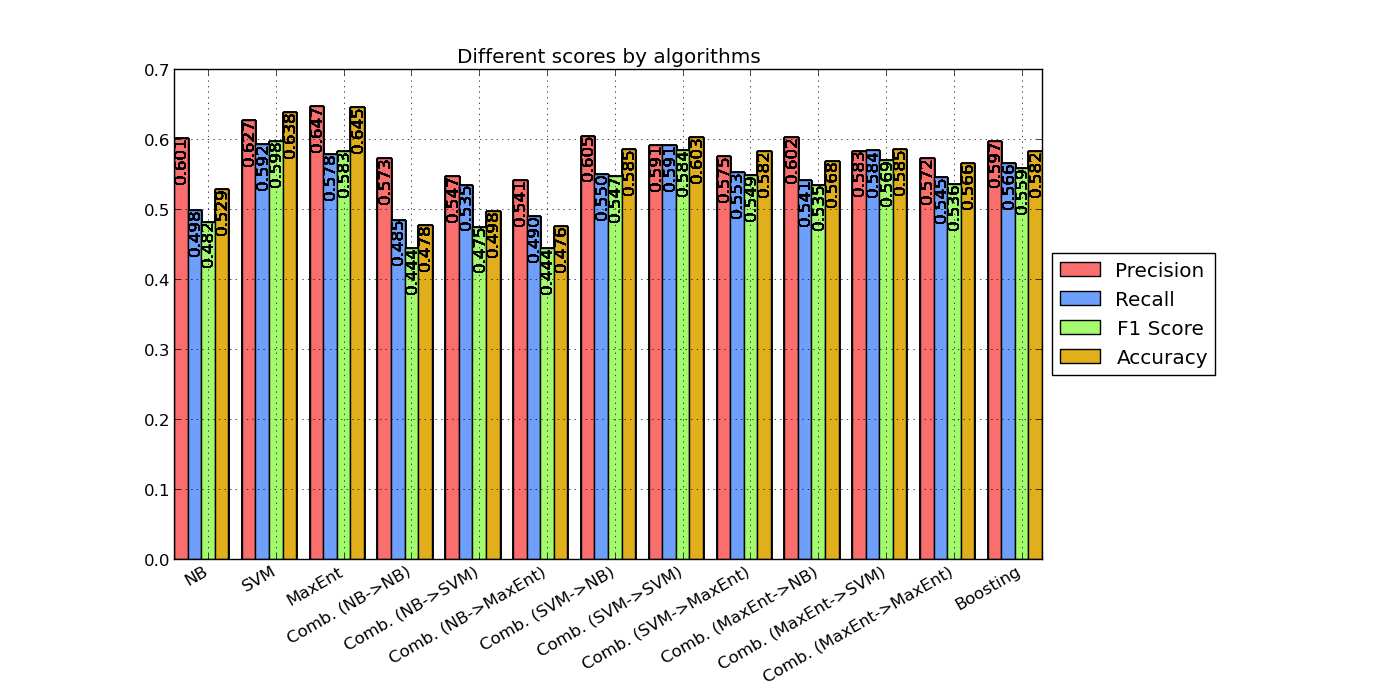
\includegraphics[width=\linewidth]{../img/plots/grid/full.png}
 \end{center}
 \caption[Results overview across models]{Caption description over here.}
 \label{fig:results_full}
\end{sidewaysfigure}


\begin{figure}[ht]
 \begin{center}
     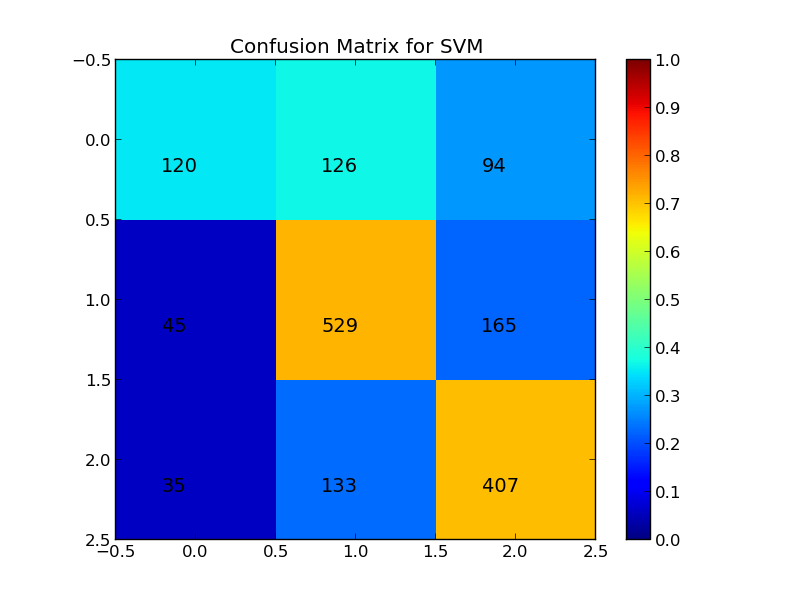
\includegraphics[width=0.7\linewidth]{../img/plots/grid/confusion_matrix_SVM.png}
 \end{center}
 \caption[Results overview across models]{Caption description over here.}
 \label{fig:confmat_svm}
\end{figure}

\begin{figure}[ht]
 \begin{center}
     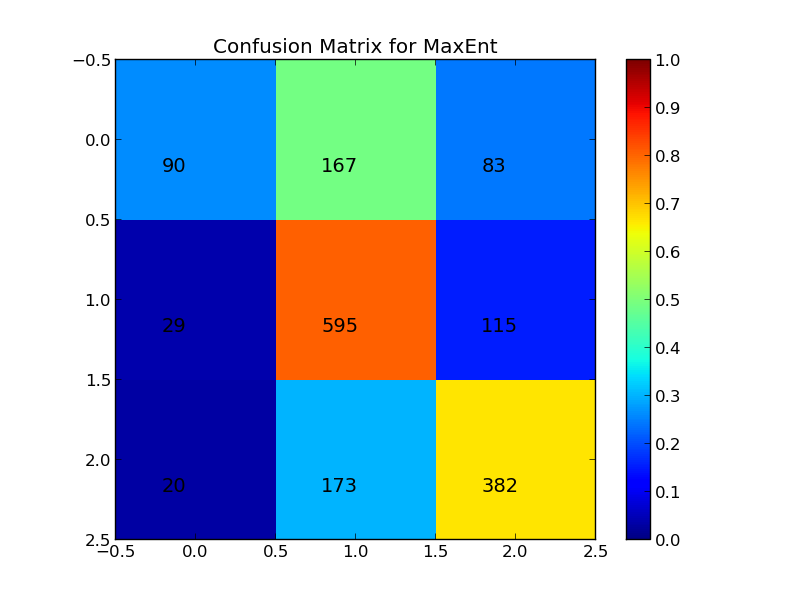
\includegraphics[width=0.7\linewidth]{../img/plots/grid/confusion_matrix_MaxEnt.png}
 \end{center}
 \caption[Results overview across models]{Caption description over here.}
 \label{fig:confmat_maxent}
\end{figure}

\begin{figure}[ht]
 \begin{center}
     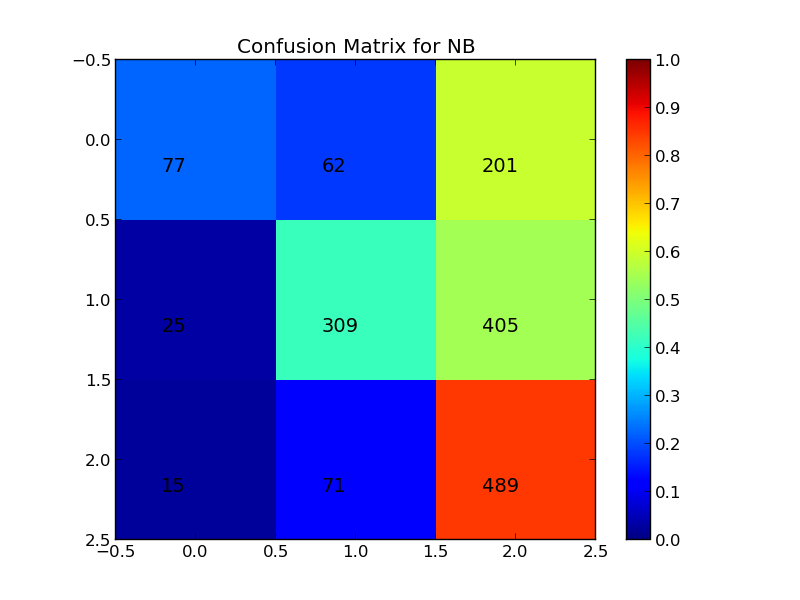
\includegraphics[width=0.7\linewidth]{../img/plots/grid/confusion_matrix_NB.png}
 \end{center}
 \caption[Results overview across models]{Caption description over here.}
 \label{fig:confmat_nb}
\end{figure}
